\chapter{Completamiento de Trayectorias en La Habana}\label{chapter:implementation}

El presente capítulo tiene como objetivo aplicar el modelo TrajBERT al conjunto de datos de telefonía móvil de Cuba para abordar el problema del completamiento de trayectorias. En particular, se busca inferir puntos faltantes en las trayectorias a partir de datos parciales y explorar su utilidad en este contexto específico.

Para ello, primero se realiza un análisis exploratorio del conjunto de datos, describiendo sus características principales y los desafíos específicos relacionados con trayectorias incompletas. A continuación, se presentan los resultados de la aplicación del modelo, destacando los casos de éxito y los retos encontrados. Por último, se comparan estos resultados con un estudio similar realizado previamente en Cuba, analizando las diferencias metodológicas y los aportes del enfoque propuesto.

\section{Descripción de los datos de ETECSA}

Para esta investigación se utilizaron los registros de actualización de área (\textit{Location Area Updates}, LAU) recopilados por la Empresa de Telecomunicaciones de Cuba (ETECSA) en La Habana durante dos meses: diciembre de 2021 y enero de 2022. Los LAU son registros generados por la red para mantener la funcionalidad del serivicio telef\'onico m\'ovil. Los mismos cuentan con tres campos de importancia para el estudio de la movilidad poblacional: un campo de ID de usuario ({\it hasheado}), un registro de tiempo y un identificador de la torre telef\'onica que est\'a en contacto con el dispositivo m\'ovil en dicho instante.

Dichos datos se almacenan de forma anonimizada, y son compartidos en los servidores de la Empresa ETECSA con los investigadores del Centro de Sistemas Complejos con fines de investigaci\'on cient\'ifica. Para mayor seguridad, en el curso de esta investigaci\'on no se usaron los datos originales anonimizados a nivel de torres, sino un posprocesado que carece de indentificador de usuario (anonimizado o no) y que tiene la ubicaci\'on proyectada en las zonas de transporte, en lugar de las torres telef\'onicas.

A diferencia de los datos usados en el cap\'itulo precedente, los datos de LAU son una fuente muy imprecisa de localizaci\'on de los usuarios de la telefon\'ia m\'ovil. En primer lugar, la posici\'on est\'a inferida a partir de la localizaci\'on de la torre telef\'onica que deja el registro correspondiente, lo cual introduce una incertidumbre de varios cientos de metros o a veces kil\'ometros. Por otro lado, la granularidad temporal tampoco es alta, y es normal encontrar registros que distan en decenas de minutos, a veces horas. Por todos estos motivos, las trayectorias que se obtienen de los registros LAU son muy ruidosas e incompletas, constituyendo un ejemplo real de utilidad para los algoritmos de completamiento de trayectorias.

A partir de estos registros se escogi\'o la siguiente definici\'on operativa de viaje:

\begin{definition}{Viaje:} Secuencia de puntos que conforman una trayectoria, de forma tal que cada par de puntos consecutivos están separados por una distancia mayor a 2 km, garantizando que no se hayan realizado paradas superiores a una hora en ninguna de los puntos de la secuencia.
\label{def:trip} \end{definition}

En el contexto cubano, la definición \ref{def:trip} resulta adecuada para describir los viajes realizados mediante transporte público. Esto se fundamenta en el hecho de que los desplazamientos a pie o en vehículos privados en La Habana rara vez exceden la hora de duración.

Para cada usuario, se procesaron los registros diarios con el objetivo de identificar viajes. Posteriormente, las secuencias de celdas obtenidas fueron mapeadas a las 134 zonas de transporte en las que el Ministerio de Transporte divide la ciudad. El mapeo se realiza asignando a cada zona de transporte un grupo de zonas de cobertura correspondientes a agrupaciones de torres con ubicaciones geográficas que se solapan. En la figura \ref{fig:havana_representation} se muestra, con líneas azules, las zonas de cobertura, y sobre ellas, con líneas rojas, las zonas de transporte.

\begin{figure}[!htb] \centering 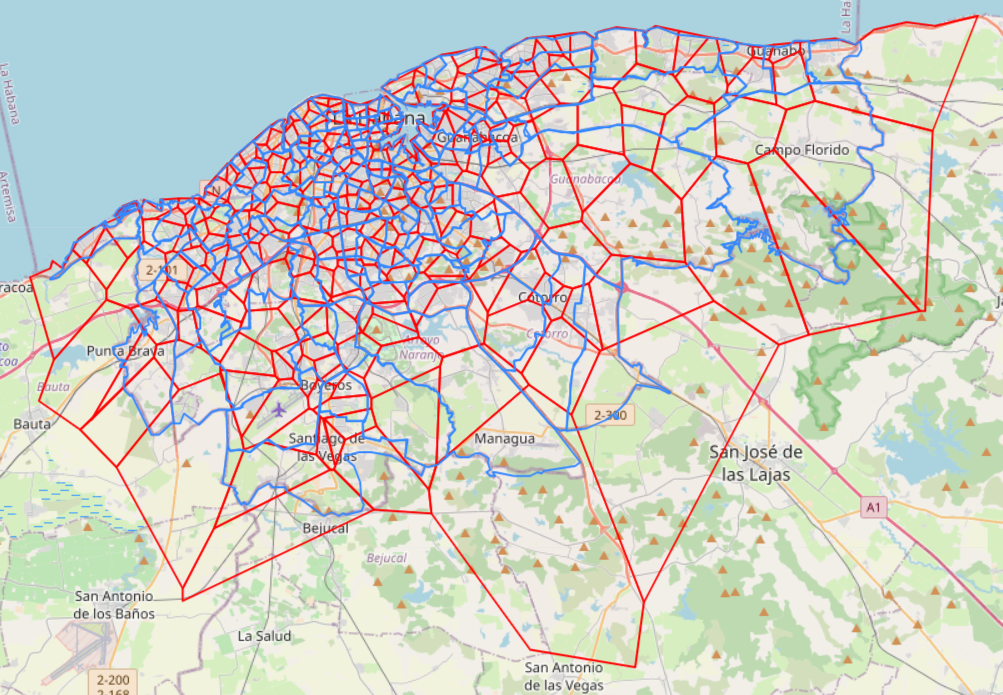
\includegraphics[width=0.9\textwidth]{Graphics/havana_representation.png} \caption{Zonas de transporte de La Habana sobre las zonas de coberturas originadas a partir de los centros de los grupos de torres.} \label{fig:havana_representation} 
\end{figure}

\begin{table}[h!]
\centering
\begin{tabular}{|p{4cm}|p{5cm}|p{5cm}|}
\hline
\textbf{Zonas}        & \textbf{Llegada}               & \textbf{Salida}                \\ \hline
[87, 106, 108, 113]   & [1013, 33742, 34979, 35340]    & [30761, 33742, 34979, 35340]   \\ \hline
[80, 33, 48, 128]     & [29818, 60456, 60527, 61743]   & [60009, 60456, 60527, 61826]   \\ \hline
\end{tabular}
\caption{Secuencias de zonas de transporte y tiempos asociados de entrada y salida a cada zona de transporte en dos viajes.}
\label{tabla:havana_data_format}
\end{table}

Esta metodología de identificación de trayectorias se ha implementado previamente en \cite{garciaborroto2021}, donde se demuestra que las trayectorias extraídas presentan una buena correlación con la información conocida sobre la movilidad en La Habana.

Como cada usuario puede dejar m\'ultiples registros en una misma zona de transporte, se decidi\'o reducir el tama\~no de los datos a partir de identificar exclusivamente la hora en la que se deja la primera se\~nal en una zona (entrada) y la hora en la que se deja la \'ultima (salida), evitando poner todos los registros intermedios. Para cada viaje, se registra la secuencia de zonas de transporte visitadas, así como los tiempos de llegada y salida correspondientes. El tiempo se codifica como un número entero que representa el segundo del día (donde 12:00:01 a.m. corresponde al número 1). De este modo, la información de los viajes se organiza en documentos con líneas formateadas como en la tabla \ref{tabla:havana_data_format}.

\subsection{Caracterización y plausiblidad de los datos}
\label{etecsa_data_description}

Los datos utilizados corresponden al registro del movimiento de usuarios desconocidos durante un período de 54 días consecutivos de actividad normal, comprendido entre el 4 de diciembre de 2021 y el 26 de enero de 2022. La figura \ref{fig:trips_per_day} refleja la dinámica temporal del número de viajes por dia y  se observa claramente una disminución en la actividad cercana a fin de año. Durante este período, la situación del Covid-19 en Cuba era relativamente favorable, lo que sugiere que estos registros de movilidad reflejan un comportamiento representativo y confiable. Inicialmente, se recopilaron un total de 6,456,967 trayectorias a lo largo de los días del estudio. En la figura \ref{fig:trip_duration_histogram} se observa que las trayectorias analizadas presentan una amplia variabilidad en sus duraciones, abarcando desde menos de una hora hasta un día completo. Asimismo, se identificaron paradas que alcanzan incluso las 5 horas de duración. Por esta razón, los datos fueron procesados para garantizar que cumplieran con la definición de viajes establecida en \ref{def:trip}.

\begin{figure}[!htb]
\centering
\begin{minipage}{0.45\textwidth}
    \centering
    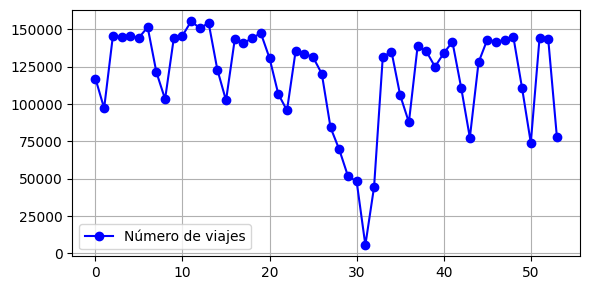
\includegraphics[width=\textwidth]{Graphics/trips_per_day.png}
    \caption{Dinámica temporal del número de viajes por día.}
    \label{fig:trips_per_day}
\end{minipage}%
\hfill
\begin{minipage}{0.45\textwidth}
    \centering
    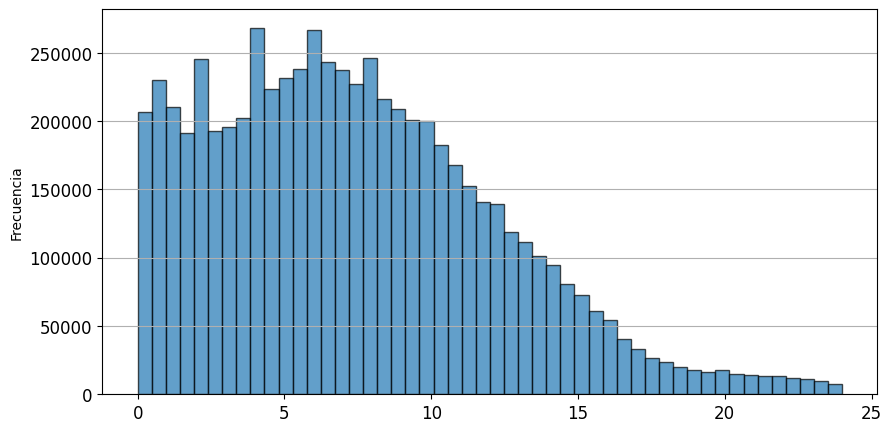
\includegraphics[width=\textwidth]{Graphics/trip_duration_histogram.png}
    \caption{Histograma de frecuencia de las duraciones de los viajes.}
    \label{fig:trip_duration_histogram}
\end{minipage}%
\end{figure}

En la figura \ref{fig:trips_per_timeslot_plot} se observa la distribución de los registros de viajes según la hora de inicio (verde) y la hora de finalización (azul). El gráfico ilustra un comportamiento coherente con los patrones de movilidad urbana: los usuarios tienden a salir en horarios específicos, y sus llegadas suelen ocurrir poco después, reflejando un desplazamiento lógico en el tiempo.

El primer pico de salidas ocurre alrededor de las 6:00 a.m., coincidiendo con el inicio típico de la jornada laboral y escolar. Este pico es seguido de cerca por un incremento en las llegadas, que alcanza su punto máximo alrededor de las 8:00 a.m., lo que sugiere que los desplazamientos durante este horario están vinculados principalmente a traslados hacia centros de trabajo o estudio. Un patrón similar se observa en la tarde: hay un segundo pico importante de salidas entre las 4:00 p.m. y las 5:00 p.m., seguido por un aumento en las llegadas hacia las 6:00 p.m., lo que refleja el regreso a casa al finalizar la jornada.

La clara sincronización entre los horarios de inicio y finalización de los viajes sugiere que los registros reflejan de manera precisa la dinámica diaria de la ciudad. Este patrón proporciona una base sólida para delimitar una ventana de estudio entre las 6:00 a.m. y las 6:00 p.m., ya que dicho intervalo concentra los períodos de mayor actividad y reduce la influencia de registros menos representativos, como los viajes realizados durante horarios nocturnos.

\begin{figure}[!htb] \centering 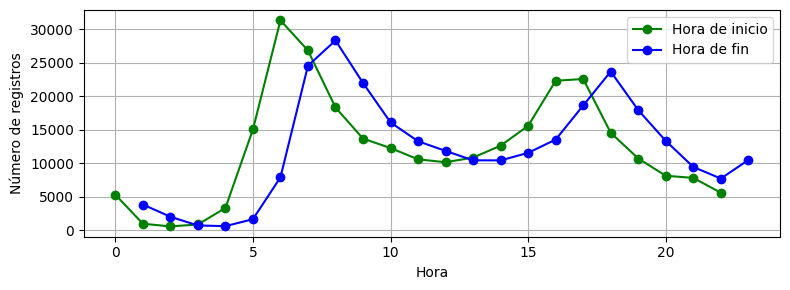
\includegraphics[width=1\textwidth]{Graphics/trips_per_timeslot_plot.png} \caption{Horas de inicio y fin de viajes agregadas en todos los días.} \label{fig:trips_per_timeslot_plot} 
\end{figure}

La figura \ref{fig:register_per_trip_histogram} muestra la distribución de la cantidad de registros por viaje tras filtrar los datos para considerar únicamente los viajes realizados entre las 6:00 a.m. y las 6:00 p.m. Se observa que la mayoría de los viajes tienen entre 4 y 6 registros, mientras que la frecuencia disminuye progresivamente a medida que aumenta el número de registros, lo que indica que los viajes más largos o complejos son menos comunes. Esto resalta que la mayoría de los trayectos son breves en cuanto a la cantidad de puntos registrados, aunque también se incluyen casos de mayor duración. La figura \ref{fig:delta_t_histogram} muestra la distribución de los tiempos entre registros consecutivos en las trayectorias analizadas. La mayoría de los intervalos son cortos, con una mediana de 12.12 minutos y una media ligeramente superior de 18.26 minutos. 

\begin{figure}[!htb]
\centering
\begin{minipage}{0.45\textwidth}
    \centering
    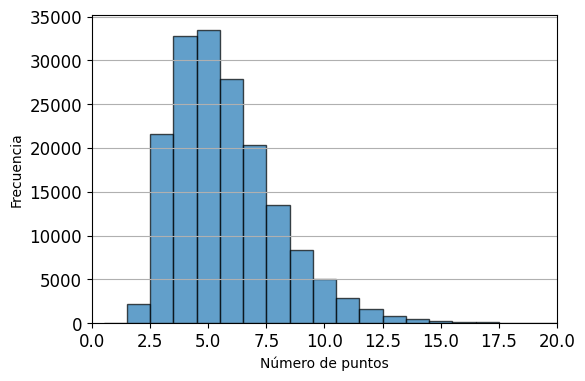
\includegraphics[width=\textwidth]{Graphics/register_per_trip_histogram.png}
    \caption{Histograma de la cantidad de registros por viajes.}
    \label{fig:register_per_trip_histogram}
\end{minipage}%
\hfill
\begin{minipage}{0.45\textwidth}
    \centering
    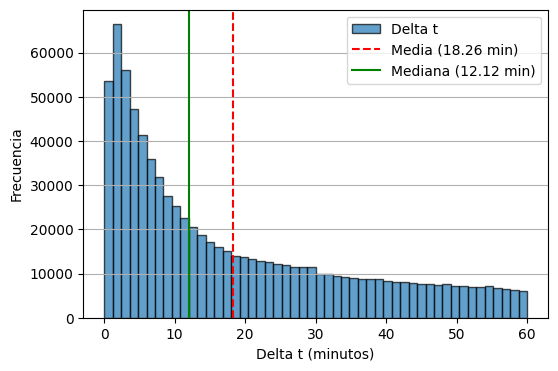
\includegraphics[width=\textwidth]{Graphics/delta_t_histogram.png}
    \caption{Distribución de los intervalos de tiempo ($\Delta t$) entre registros consecutivos.}
    \label{fig:delta_t_histogram}
\end{minipage}%
\end{figure}

Por último, se realizó un análisis de las diferencias en los flujos de transporte entre la mañana y la tarde, evidenciando un patrón de movilidad típico de áreas metropolitanas, como se muestra en la figura \ref{fig:morning_afternoon_difference_coulor}. En la mañana, las zonas periféricas registran un mayor flujo de salidas, representadas por tonos claros, mientras que las zonas centrales, de mayor actividad socioeconómica, muestran un aumento en las llegadas, reflejado en tonos oscuros. Esto evidencia el desplazamiento de personas desde sus hogares hacia zonas de trabajo o servicios. Por el contrario, en la tarde, el flujo se invierte: las personas regresan a sus zonas de residencia en la periferia, mientras que las zonas centrales pierden afluencia. Estos patrones son coherentes con los datos de movilidad previamente observados en La Habana y reportados en \cite{padron2021transporte}.

\begin{figure}[!htb] \centering 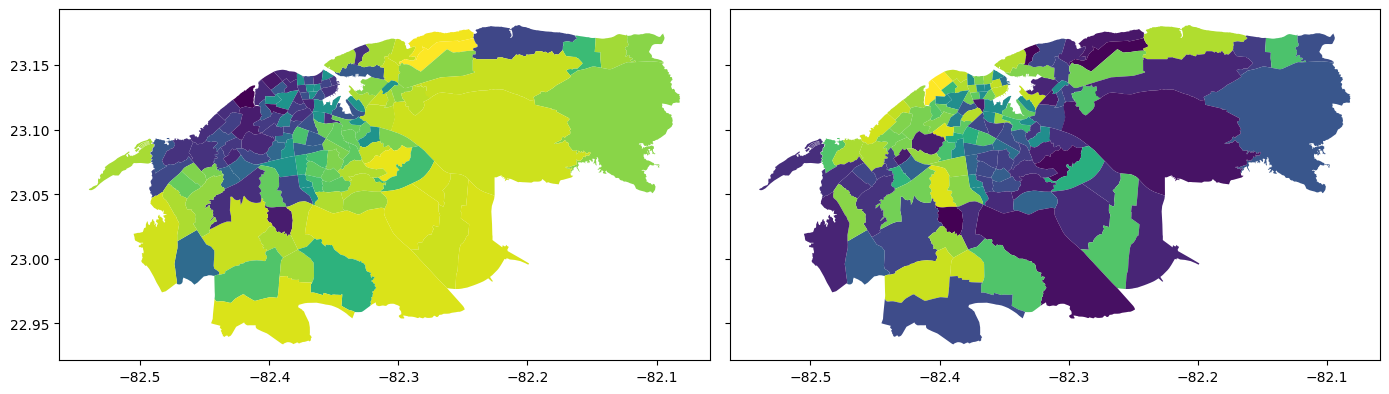
\includegraphics[width=1\textwidth]{Graphics/morning_afternoon_difference_coulor.png} \caption{Diferencia entre salidas y llegadas por zona de transporte: tonos claros indican más salidas, oscuros más llegadas. Izquierda: mañana, derecha: tarde.} \label{fig:morning_afternoon_difference_coulor} 
\end{figure}

En términos generales, los datos son consistentes con investigaciones previas y con el conocimiento que tenemos sobre la ciudad y su dinámica. Esto nos permite asumir que la definición de viajes utilizada es adecuada y captura de manera precisa la movilidad poblacional en La Habana durante el período analizado. En la sección siguiente, aplicamos la metodología propuesta en el capítulo anterior para el completamiento de estas trayectorias.

\section{Experimentación y resultados}

Este experimento tiene como objetivo principal ajustar los hiperparámetros del modelo TrajBERT para optimizar su desempeño sobre los datos de telefonía móvil cubanos. Además, se buscó comparar los resultados obtenidos con un estudio similar realizado recientemente en La Habana, evaluando cómo el modelo podría capturar las relaciones espaciales y temporales específicas de la región.

\begin{figure}[!htb] \centering \includegraphics[width=0.7\textwidth]{Graphics/data_preproccess_flow.pdf} \caption{Ilustraci\'on del proceso de transformaci\'on de los datos en tiempo continuo de los registros LAU al formato requerido por TrajBERT.} \label{fig:data_preproccess_flow} 
\end{figure}

El primer paso fue adaptar el formato de los datos de telefonía móvil cubanos, ver tabla \ref{tabla:havana_data_format}, al formato de entrada de TrajBERT. Para ello, se desarrolló un proceso de transformación que agrupó los datos por viaje, generando trayectorias de longitud fija. Durante este proceso, se asignó a cada intervalo el valor más frecuente de la ubicación registrada como se ilustra en el diagrama 
\ref{fig:data_preproccess_flow}. La distribución observada en \ref{fig:delta_t_histogram} respalda la elección de $\epsilon$, definido en \ref{def:e_sampling}, como 15 minutos, ya que permite capturar la mayoría de los registros frecuentes sin generar redundancia ni perder información relevante sobre las trayectorias. Por lo tanto, para estos datos se tomó $m = 48$, similar a lo hecho en la sección \ref{sec:humob_experiments} y en el trabajo original \cite{si2023trajbert}. 

Los datos fueron particionados con la misma proporción que en la sección \ref{sec:humob_experiments}. El modelo fue entrenado utilizando un equipo de cómputo de alto rendimiento equipado con una tarjeta gráfica NVIDIA GeForce RTX 4090, que cuenta con 24 GB de memoria dedicada y soporte para CUDA 12.7, ofreciendo capacidades excepcionales para cálculos intensivos y entrenamiento de modelos de aprendizaje automático.  

Sobre el conjunto de validación se observó que el rendimiento del modelo mejoraba al incrementar el tamaño del \textit{embedding}, pero comenzaba a decrecer una vez superado un tamaño de 512. Por ello, se seleccionó 512 como el tamaño óptimo para este caso. Además, se identificó que aumentar el número de capas y cabezas de atención disminuía el rendimiento del modelo, lo cual puede atribuirse a que la estructura de las trayectorias son más simples en comparación con datos secuenciales más complejos, como el lenguaje natural. Los patrones de movilidad en la ciudad son periódicos y están limitados por la estructura espacial urbana, lo que implica relaciones estables y simples entre las ubicaciones. Por este motivo, se decidió configurar el modelo con dos capas y dos cabezas de atención, priorizando su capacidad de generalización en este contexto específico. En la figura \ref{fig:etecsa_hiperparameter_variability} se puede observar lo antes mencionado.

\begin{figure}[!htb] \centering 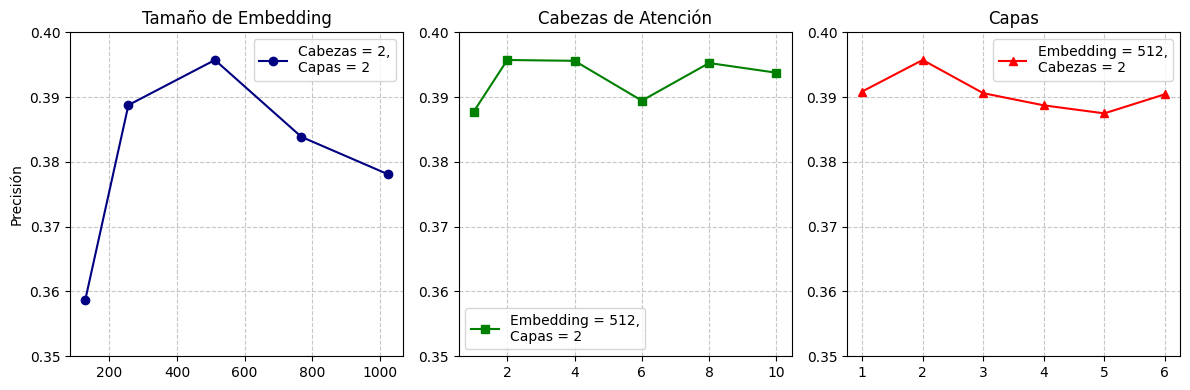
\includegraphics[width=1\textwidth]{Graphics/etecsa_hiperparameter_variability.png} \caption{Relación entre la exactitud y los valores de tamaño del \textit{embedding}, número de cabezas de atención, y número de capas. Los valores de \textit{embedding}, cabezas y capas están fijados en 512, 2 y 2 respectivamente, excepto en la gráfica correspondiente donde se analiza su variación.} \label{fig:etecsa_hiperparameter_variability} 
\end{figure}

El modelo logró una exactitud base de 39.60\% en la clasificación directa sobre el conjunto de prueba, demostrando capacidad inicial de aprendizaje en condiciones reales. Al incorporar métricas de evaluación extendidas, se observa un progreso significativo: la métrica \textit{fuzzy-acc} alcanza 57.19\%, mientras que los resultados en \textit{top-3}, \textit{top-5} y \textit{top-10} muestran valores de 58.87\%, 62.83\% y 68.51\% respectivamente, lo que indica una tendencia positiva en la identificación de patrones espaciales. En cuanto a la precisión geográfica, la distancia promedio entre predicciones y valores reales fue de 3.82 km, un resultado inicial que establece un punto de referencia para optimizaciones futuras.

Para evaluar el impacto de la completitud de los datos en el modelo, se introdujo el concepto de densidad de trayectorias, definido como la proporción de puntos conocidos respecto a la longitud total de la secuencia (excluyendo los tokens de \textit{padding} en los extremos). El análisis de la densidad de trayectorias reveló patrones clave sobre la adaptabilidad del modelo.

Las trayectorias del conjunto de prueba se clasificaron en tres niveles: baja (<50\% de datos conocidos), media (50\%-80\%) y alta (>80\%). Como se observa en la figura \ref{fig:accuracy_metrics}, existe una correlación positiva entre completitud y desempeño: la exactitud aumentó de 36.60\% en trayectorias de baja densidad a 44.43\% en aquellas de alta densidad. Además, las métricas extendidas mostraron una mayor resiliencia, con un \textit{top-10} que alcanzó el 78.20\% en trayectorias de alta densidad y se mantuvo en 61.68\% incluso en secuencias con baja densidad. Complementando este análisis, la figura \ref{fig:geospatial_distance} muestra que la distancia geoespacial promedio disminuyó progresivamente con el aumento de la densidad, evidenciando que las trayectorias más completas permiten una localización más precisa.

\begin{figure}[!htb]
\centering
\begin{minipage}{0.45\textwidth}
    \centering
    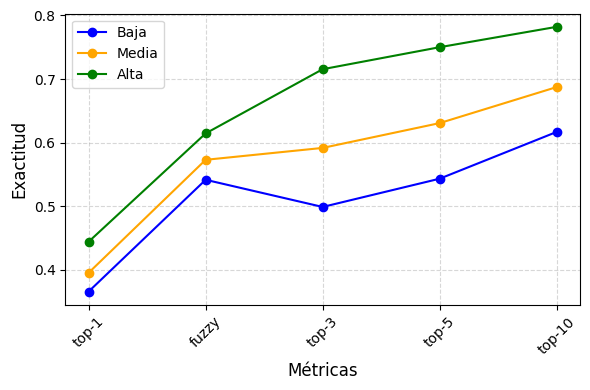
\includegraphics[width=\textwidth]{Graphics/accuracy_metrics.png}
    \caption{Comportamiento de las métricas de exactitud al variar las densidades.}
    \label{fig:accuracy_metrics}
\end{minipage}%
\hfill
\begin{minipage}{0.45\textwidth}
    \centering
    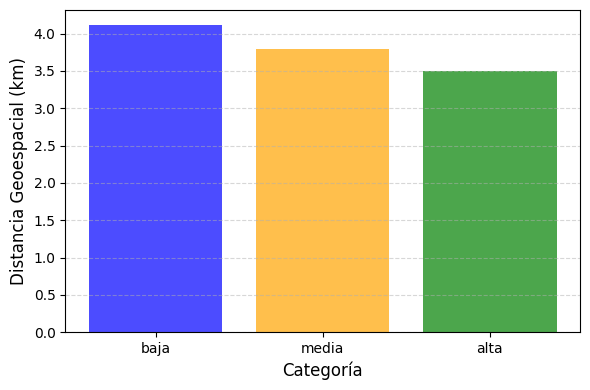
\includegraphics[width=\textwidth]{Graphics/geospatial_distance.png}
    \caption{Comportamiento de la distancia geoespacial promedio al variar las densidades.}
    \label{fig:geospatial_distance}
\end{minipage}%
\end{figure}

Los resultados muestran que, si bien la densidad de datos afecta el desempeño del modelo, este sigue siendo capaz de sugerir ubicaciones geográficas plausibles, evidenciando su potencial en análisis de movilidad a gran escala. No obstante, al procesar puntos de forma aislada en contextos de alta incertidumbre se pierden las dependencias espaciotemporales, lo que incrementa los errores y reduce la efectividad. Esto valida que la integración del contexto secuencial optimiza el manejo de datos fragmentados.

Para dar sentido relativo a estos resultados, en el siguiente ep\'igrafe se comparan con los obtenidos usando otro esquema m\'as simple de redes neuronales.

\section{Completamiento de trayectorias con ANN}

En la revisión bibliográfica, se identificaron varios estudios \cite{rodriguez2022movilidad, padron2021transporte, garciaborroto2021, durive2021sistema} que abordan el uso de datos de telefonía móvil para identificar patrones de movilidad en Cuba. En particular, uno de ellos propone un modelo basado en redes neuronales artificiales para la \textit{Reconstrucción de Trayectorias en Puntos Intermedios} (IPPR, por sus siglas en inglés) \cite{rodriguez2022movilidad}. Este modelo predice la ubicación intermedia de un viajero a partir de su origen, destino y una fracción del trayecto completada.

El modelo recibe como entrada cinco valores: la latitud y longitud del punto de origen, la latitud y longitud del destino, y un valor en el intervalo $[0,1]$ que representa el progreso del viaje. La salida es una distribución de probabilidad sobre 134 zonas de transporte, obtenida mediante una capa \textit{softmax}. La red neuronal emplea una arquitectura de tres capas ocultas totalmente conectadas, ver figura \ref{fig:ann_architecture}. El entrenamiento del modelo se realizó utilizando el optimizador Adam, minimizando la divergencia de Kullback-Leibler \cite{van2014renyi}.

\begin{figure}[!htb]
\centering
\begin{minipage}{0.50\textwidth}
    \centering
    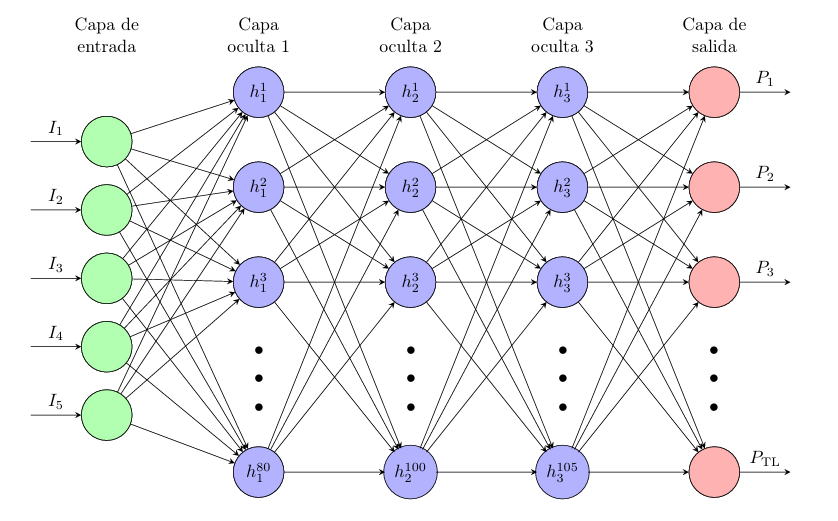
\includegraphics[width=\textwidth]{Graphics/ann_architecture.png}
    \caption{Arquitectura de la ANN para la \textit{Reconstrucción de Trayectorias en Puntos Intermedios}, figura extraída de \cite{rodriguez2022movilidad}.}
    \label{fig:ann_architecture}
\end{minipage}%
\hfill
\begin{minipage}{0.45\textwidth}
    \centering
    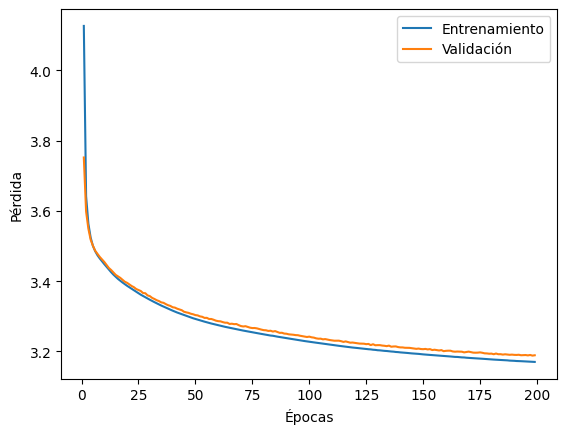
\includegraphics[width=\textwidth]{Graphics/ann_loss.png}
    \caption{Comportamiento de la función de pérdida en los conjuntos de entrenamiento y validación.}
    \label{fig:ann_loss}
\end{minipage}%
\end{figure}

Establecer una comparación directa entre TrajBERT y los resultados expuestos en \cite{rodriguez2022movilidad} resulta muy difícil, ya que, aunque ambos modelos fueron entrenados con el mismo conjunto global de datos, el filtrado y la segmentación aplicados fueron diferentes. En \cite{rodriguez2022movilidad} se trabajó únicamente con registros tomados de 6:00 a.m. a 10:00 a.m., y se presentan resultados luego de dividir el conjunto de prueba en tres subconjuntos en función de la distancia entre los \textit{ID de ubicación} de origen y destino de cada trayectoria. Esta estrategia difiere evidentemente de la empleada en este trabajo, lo que imposibilita una comparación directa de los desempeños reportados.

Por lo tanto, con el fin de comparar el modelo propuesto en \cite{rodriguez2022movilidad} con los resultados de TraBERT, se optó por reentrenar la ANN utilizando las mismas especificaciones propuestas, pero esta vez con los datos descritos en la sección \ref{etecsa_data_description}. El objetivo era partir de la misma base de conocimiento para ambos modelos, permitiendo así una comparación justa en términos de capacidad de generalización y desempeño. En la figura \ref{fig:ann_loss} se muestra el comportamiento de la función de pérdida en los conjuntos de entrenamiento y validación durante 200 épocas, mostrando cómo el modelo converge consistentemente.

\subsection{Comparación con TrajBERT}

Aunque el modelo propuesto en \cite{rodriguez2022movilidad} resulta ingenioso, presenta una limitación crítica: no aprovecha de manera adecuada la información contextual inherente a las trayectorias secuenciales. Las trayectorias urbanas no son simplemente colecciones de puntos aislados, sino secuencias espaciotemporales en las que la elección de una zona de transporte depende de decisiones previas y de patrones de movilidad subyacentes. La arquitectura de la ANN, al procesar cada cuadrupleta (origen, intermedio, destino, fracción de tiempo) de forma independiente, ignora las dependencias a largo plazo y la estructura secuencial que modelos como TrajBERT capturan mediante mecanismos de atención.

Los resultados numéricos de la tabla \ref{tab:etecsa_model_comparison} reflejan esta brecha. Mientras la ANN alcanza una exactitud del 18.92\% y una distancia geográfica promedio de 4.82 km, TrajBERT duplica la exactitud (39.60\%) y reduce el error geográfico a 3.82 km. Además, en métricas que evalúan la flexibilidad de las predicciones (\textit{top-3}, \textit{top-5} y \textit{top-10}), TrajBERT supera consistentemente a la ANN, lo que sugiere una mayor capacidad para generar distribuciones de probabilidad mejor calibradas y contextualmente relevantes.

\begin{table}[ht]
\centering
\begin{tabular}{|l|c|c|c|c|c|}
\hline
\textbf{Modelo} & \textbf{Exactitud} & \textbf{top-3} & \textbf{top-5} & \textbf{top-10} & \textbf{Distancia (km)} \\ \hline
ANN             & 0.1892                & 0.3924            & 0.5122            &  0.6786            & 4.8170                  \\ \hline
TrajBert        & 0.3960                & 0.5887            & 0.6283            & 0.6851             & 3.8238                  \\ \hline
\end{tabular}
\captionof{table}{Comparación de resultados entre la ANN y TrajBERT.}
\label{tab:etecsa_model_comparison}
\end{table}

Los resultados indican que, al basarse únicamente en puntos intermedios, la ANN no logra capturar de forma efectiva la compleja estructura espacial de La Habana. En cambio, TrajBERT, gracias a su refinamiento espaciotemporal (sección \ref{trajectory_encoder}) y la función STAL (sección \ref{stal_function}), extrae patrones geográficos con mayor precisión, lo que se refleja en un desempeño superior en el completamiento de trayectorias.

Evaluar el impacto de la densidad de trayectorias en la ANN no tiene fundamentación metodológica, ya que este modelo no procesa la información en forma secuencial. Por lo tanto, las variaciones en la densidad no influyen en la comprensión de una trayectoria en particular. Sin embargo, siguiendo el enfoque de \cite{rodriguez2022movilidad}, que define la distancia origen-destino como el número mínimo de aristas entre nodos en el grafo de zonas de transporte de La Habana, nuestro análisis (ver figura \ref{fig:distance_variability}) revela que ambos modelos mantienen una estabilidad métrica frente a trayectorias de distancias crecientes, con TrajBERT mostrando un rendimiento superior. Este resultado contrasta con lo reportado en \cite{rodriguez2022movilidad}, donde se observa una degradación en la efectividad del completamiento de trayectorias más largas. Las trayectorias se clasificaron en tres niveles: corta (<6 aristas entre los nodos origen-destino), media (6-8) y lejana (>8).

\begin{figure}[!htb] \centering 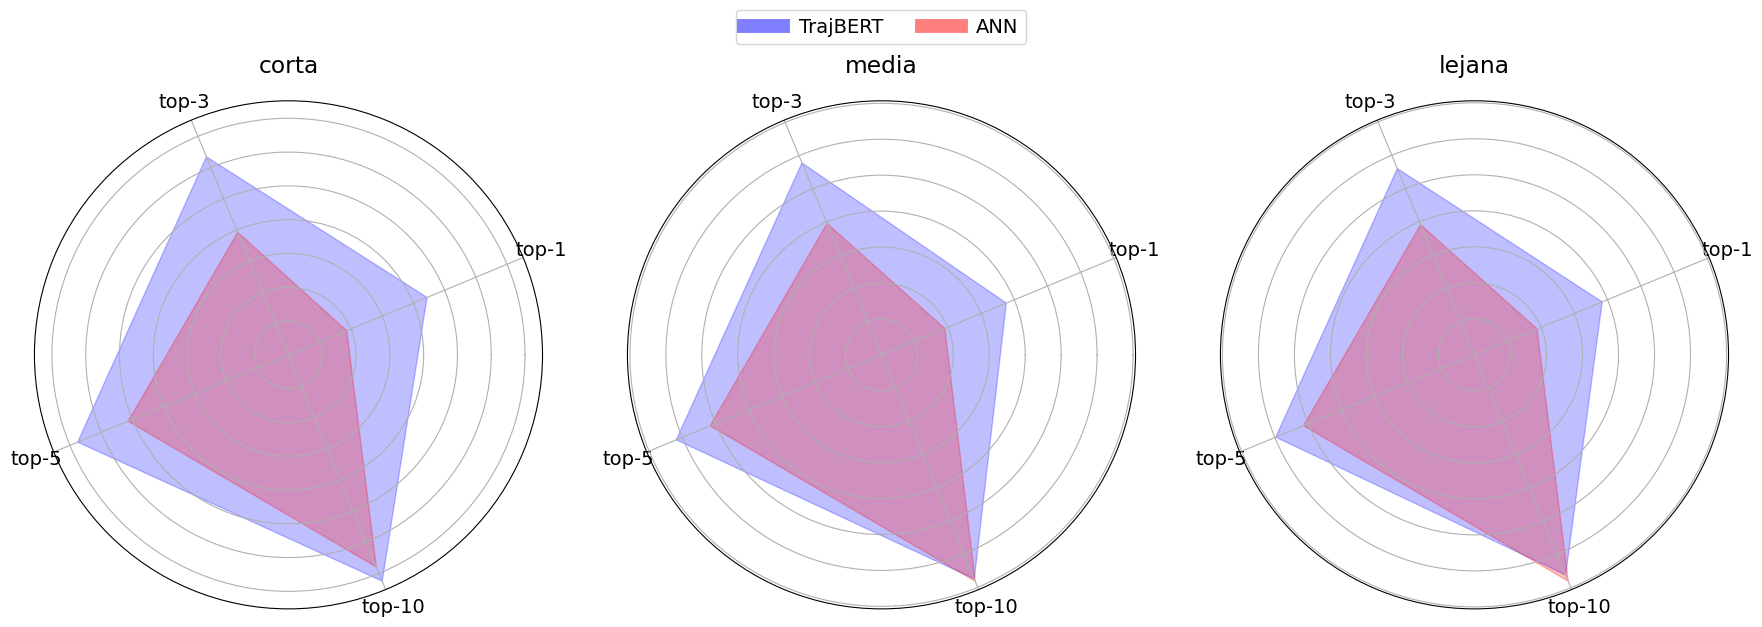
\includegraphics[width=1\textwidth]{Graphics/distance_variability.png} \caption{Comparación de las métricas de exactitud entre TrajBERT y la ANN de \cite{rodriguez2022movilidad} al variar la distancia entre los \textit{ID de ubicación} de origen y destino.} \label{fig:distance_variability} 
\end{figure}

La discrepancia en el comportamiento de la ANN puede explicarse por diferencias en la calidad o distribución de los datos y las condiciones de entrenamiento. Por lo tanto, se concluye que, al menos en este conjunto de datos, TrajBERT ofrece un desempeño significativamente superior.